\chapter{One Cell Prototype}

The work presented in this thesis is done in the framework of the One Cell Prototype.
Therefore the prototype is described in more detail in this chapter.
Although the important parts of the One Cell Prototype are all mentioned here, the main focus lies on the amplifier and the digitizer since these are the most relevant parts of this thesis.
Firstly the cell and the liquid scintillator are shown, followed by the \ac{wom} used to capture the scintillation light, the \acp{sipm} used for the light detection, and the optical coupling between the \ac{wom} and the and the \acp{sipm}, are presented afterward.
Subsequently, the amplifier and the digitizer are introduced.



\section{The Cell \& Liquid Scintillator}

In \autoref{fig:one_cell}, the One Cell Prototype is shown.
It is \SI{80}{\centi\meter} wide and around \SI{120}{\centi\meter} high.
However, the precise height depends on the position in the cell due to the asymmetric shape.
The walls of the cell consist of \SI{1}{\centi\meter} thick corten steel.
The steel was chosen because of the rather low price tag, which is an important aspect considering the size of the \ac{sbt}.
A thickness of \SI{1}{\centi\meter} is only half of the planned \SI{2}{\centi\meter} wall thickness of the \ac{sbt} design.
The \ac{sbt} needs such thick walls in order to withstand the vacuum on the inside.
For the R\&D with the One Cell Prototype, the thickness was reduced to be able to perform measurements with different wall thicknesses by adding steel plates to the outside.
This is important in case the \ac{sbt} design changes, for example by replacing the vacuum with helium.
One side of the cell has two holes with a \SI{}{\centi\meter} radius.
They have an equal distance to both side walls.
The lower hole is \SI{30}{\centi\meter} away from the bottom of the cell, and the upper hole is \SI{30}{\centi\meter} below the top.
In each of these holes, a PMMA vessel, shown in \autoref{fig:pmma_vessel}, is placed to house the two \acp{wom} and protect their wavelengthshifting coating from the liquid scintillator.
A reflective paint was applied to the inside of the cell to increase the scintillator's light yield and therefore increase the detector's efficiency.
\begin{figure}
	\centering
	\begin{subfigure}[b]{.40\textwidth}
		\centering
		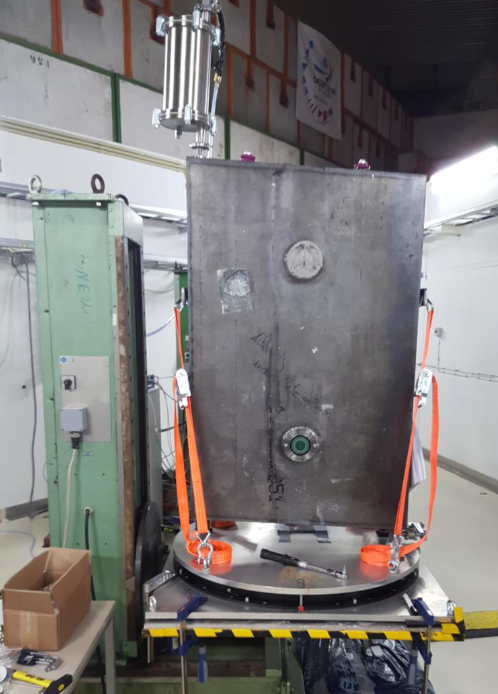
\includegraphics[width=1.\textwidth]{pictures/one_cell}
		\caption[One Cell Prototype]{}
		\label{fig:one_cell}
	\end{subfigure}
	\begin{subfigure}[b]{.54\textwidth}
		\centering
		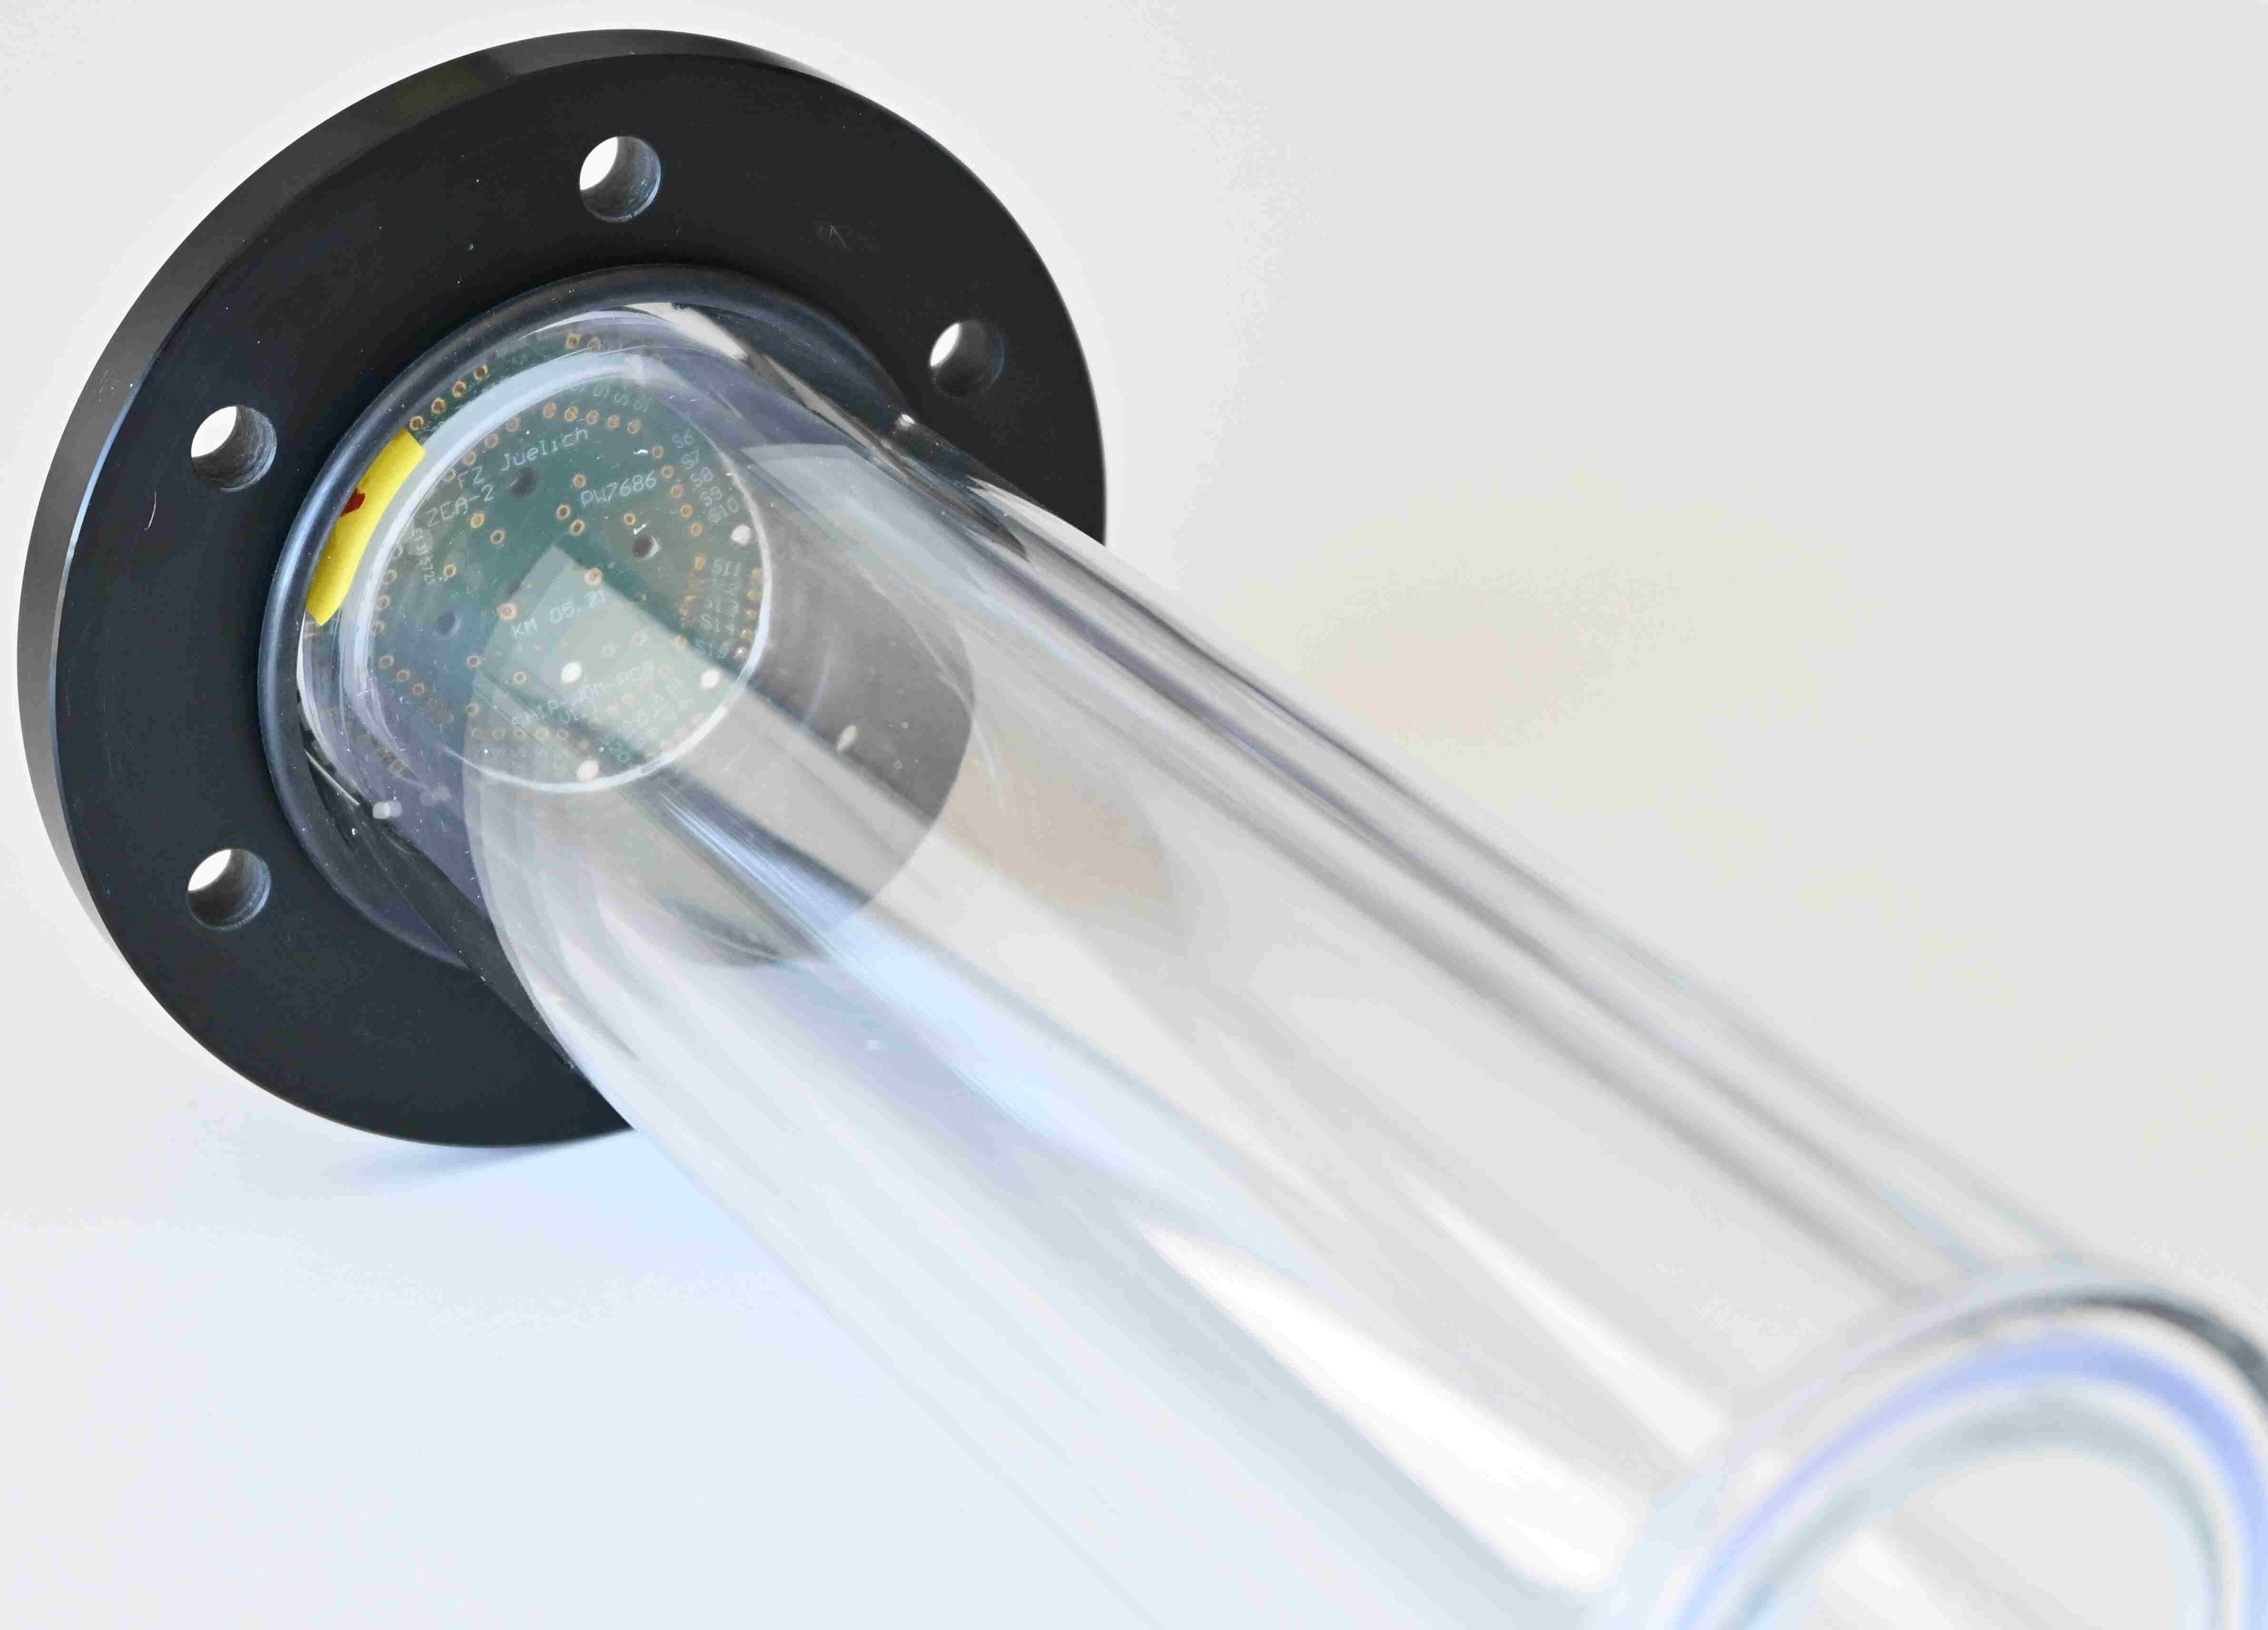
\includegraphics[width=1.\textwidth]{pictures/pmma_vessel}
		\caption[PMMA vessel]{}
		\label{fig:pmma_vessel}
	\end{subfigure}
	\caption[One Cell Prototype and PMMA vessel]{The One Cell Prototype at the DESY testbeam area a) and a PMMA vessel with a Wavelenthshifting Optical Module inserted and a \ac{sipm} board attached b). \cite{}}
	\label{fig:one_cell_and_pmma}
\end{figure}

The cell is filled with the liquid scintillator \ac{lab} mixed with \SI{2}{\gram\per\liter} Diphenyloxazole (PPO)%, which is also planed to be used in the \ac{sbt}.
In order to allow decrompression and compression by temperature change, an expansion vessel is mounted on top of the cell.
%To fill the cell \SI{}{\kilo\gram} \ac{lab} were used.
%This is around \SI{3}{\kilo\gram} more than the amount fitting into the cell.
%The extra \ac{lab} is in the expansion vessel, in order for the cell still being full in case of a temperatur decline and compession of the \ac{lab}.
The cell was overfilled with scintillator, in order to still being full if the temperature declines and the scintillator compresses.
Gaseous nitrogen fills out the remaining volume of the expansion vessel to serve as a compressible volume. 

\ac{lab}s emission spectrum is shown in \autoref{fig:lab_emission}.
Most of the scintillation light has a wavelength of \SIrange{320}{360}{\nano\meter}.
In order to capture the light and to shift the wavelength towards values for which the used \acp{sipm} have a higher detection efficiency, \acp{wom} are used.
In the next section, these \acp{wom} and the optical coupling between them and the \acp{sipm} are presented.
\begin{figure}
	\centering
	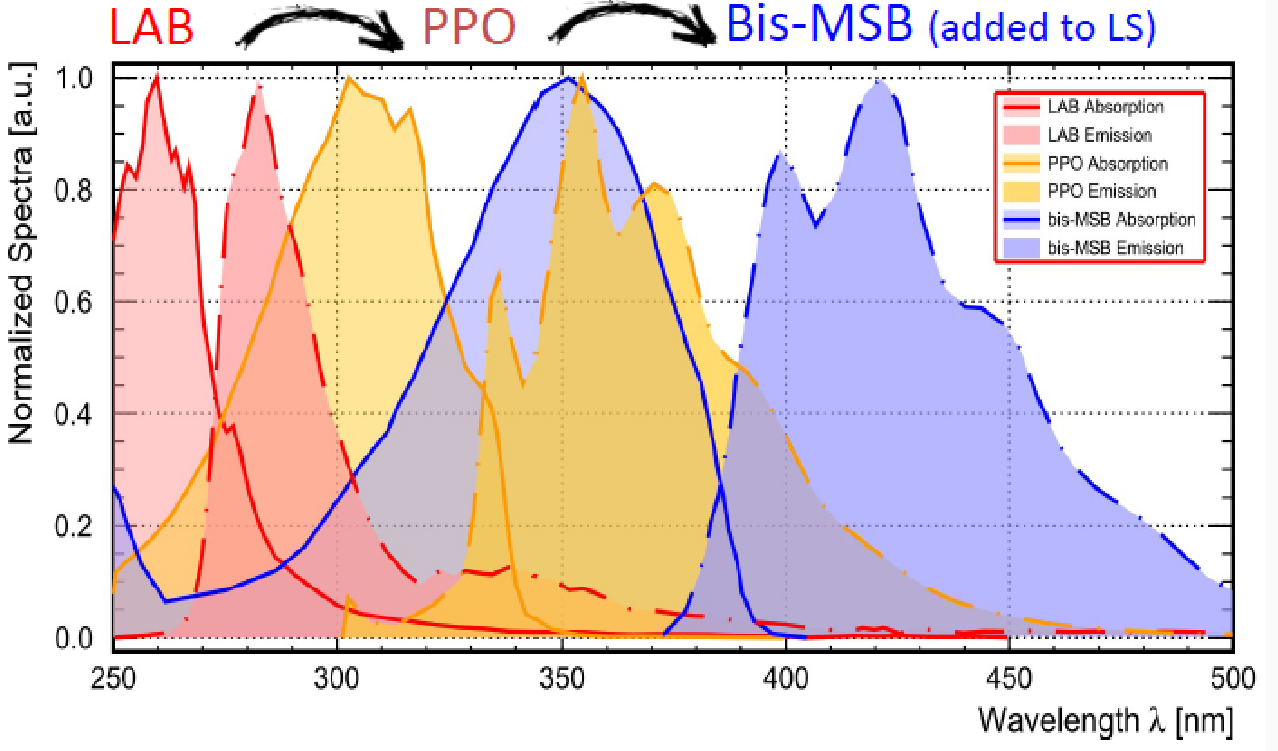
\includegraphics[width=.8\textwidth]{pictures/lab_emission}
	\caption[LAB emission spectrum]{The emission spectrum of the liquid scintillator components \ac{lab} and \ac{ppo} and the wavelength shifter Bis-MSB. \cite{}}
	\label{fig:lab_emission}
\end{figure}



\section{Wavelengthshifting Optical Module \& Optical Coupling}

So-called \acp{wom} are used to capture the scintillation light.
They are PMMA cylinder walls with a \SI{6}{\centi\meter} outer diameter and a \SI{3}{\milli\meter} wall thickness.
The design and material choice both make the cost of the light collection relatively cheap.
Both the inside and outside of the PMMA cylinder are coated with the wavelength shifter Bis-MSB \cite{}.
So the captured photons are shifted to a higher wavelength, for which the \acp{sipm} used for the light detection have a higher efficiency.
\autoref{fig:lab_emission} shows the wavelength spectrum of the wavelength-shifted light.
The photons which enter the \ac{wom} are trapped there by total reflection on the walls.
They can leave the \ac{wom} at its end, where an array of forty \acp{sipm} can detect them.
For a good optical coupling between the \ac{wom} and the \acp{sipm}, either optical grease or silicon pads can be used.
\autoref{fig:wom_principle} illustrates the principle of the \ac{wom} with the wavelength shifting and capture by total reflection.
\begin{figure}
	\centering
	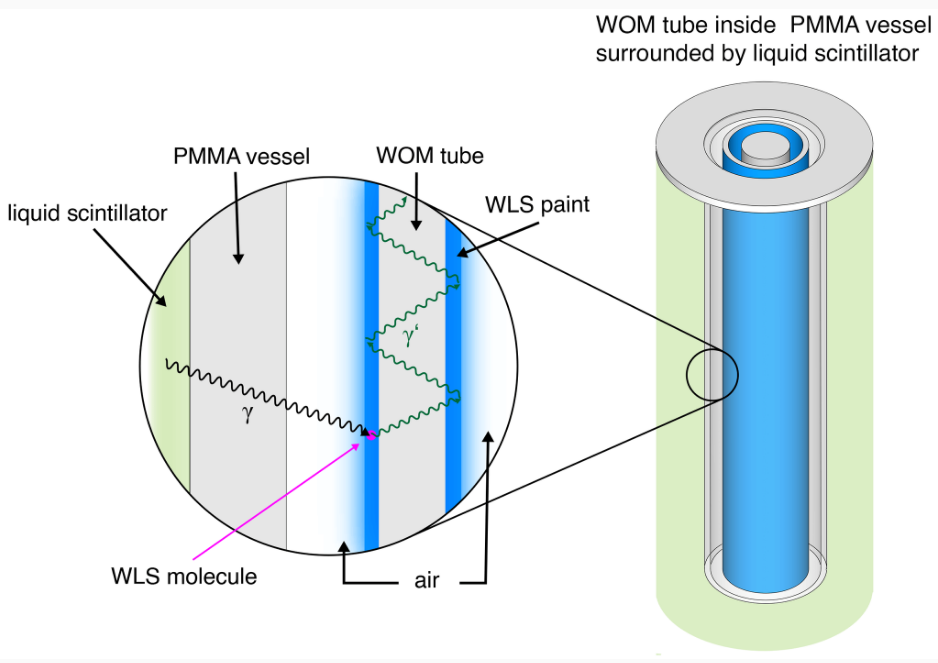
\includegraphics[width=.8\textwidth]{pictures/wom_principle}
	\caption[Working principle of a WOM]{A Wavelengthshifting Optical Module (WOM) is a PMMA tube coated with the wavelength shifter Bis-MSB. If a photon in the UV range hits the WOM, its wavelength gets shifted. Afterward, in the WOM, the photon is trapped by total reflection. At the end of the WOM, the photon can be detected by a photosensor. \cite[]}
	\label{fig:wom_principle}
\end{figure}

In the next part, the \acp{sipm}, which detect the light captured by the \acp{wom}, are presented.


\section{Silicon Photomultiplier}
In order to correctly identify and tag background events, the light detection of the \ac{sbt} has to provide accurate timing information.
Furthermore, due to the number of cells and \acp{wom} in the \ac{sbt}, it should not cost a lot per \ac{wom}.
To fulfill both requirements, \acp{sipm} were chosen as photodetectors.
These photodetectors consist of up to thousands of pixels.
Each pixel is a photodiode with a typical edge length between \SI{10}{\micro\meter} and \SI{100}{\micro\meter} \cite{nucl}.
If triggered by light, a \ac{sipm} sends out a charge signal proportional to the number of triggered pixels.
In the case that the number of incoming photons is low compared to the number of pixels, such that two photons hitting the same pixel is unlikely, the charge signal is linear to the light intensity.
The charge signal possesses a fast-rising edge with a rise time of the order of tens of \si{\piko\second} \cite{nucl}.
Besides the excellent time resolution, \acp{sipm} also make it possible to count the arriving photos with a sensitivity down to single photons \cite{HAMA_mppc}.

Each pixel in the \ac{sipm} is an \ac{spad}, which is a \ac{apd} supplied with a voltage greater than its breakdown voltage.
In the following, the principle of such an \ac{apd} and \ac{spad} are explained.

Similar to every photodiode, \ac{apd} utilize, the photoelectric effect to generate an electric charge signal in response to a light signal.
They consist of doped silicon.
An example is shown in \autoref{fig:pin_diode}.
It has a strongly n-doped layer, followed by a strongly p-doped layer, an intrinsic, weakly p-doped layer, and another p-doped layer.
By adding the intrinsic layer, the region in which the photons can be absorbed increases.
If a photon gets absorbed, it generates an electron-hole pair.
When a reversed bias voltage is applied, the electric field in the \ac{apd} separates the $eh$-pair.
In case the \ac{apd} is operated in the Geiger mode, meaning the bias voltage is higher than the breakdown voltage of the \ac{apd}, the electric field at the strongly doped $p$- and $n$-layer is sufficiently high, that a self-sustaining avalanche is triggered by either the electron or the hole moving through it.
Then the \ac{apd} is called \ac{spad}.
The macroscopic signal of a \ac{spad} makes it possible to detect single photons.
In order to stop the avalanche, a quenching resistor is connected in series to the \ac{spad}.
With an increasing current signal flowing through the quenching resistor, the voltage drop at this resistor increases, and thus the bias voltage at the \ac{spad} decreases.
When the bias voltage drops under the breakdown voltage, the avalanche is no longer self-sustaining and stops.
Thus the signal amplitude of a \ac{spad} is always similar, independent of how many photons arrive at the same moment.


%Similar to every photodiode, \acp{apd} utilize the photoelectric effect, to generate an electric charge signal in response to a light signal.
%This is made possible by using silicon as a base material and introducing impurities. 
%This process is called doping and there are two different possibilities for doping. 
%In the n-doping, the impurities are atoms with five valence electrons.
%Four of these electrons are part of boundings with silicon atoms, and the fifth electron is only weakly bound.
%When p-doping, atoms with only three valence electrons are inserted into the silicon.
%This leads to missing charges in the silicon, called holes.
%By having an n-doped and a p-doped region in the silicon, the excess electrons from the n-doped region combine with the holes from the p-doped region, resulting in a depleted region at the pn-junction.
%If a photon hits the photodiode, it can create an electron-hole pair, or $eh$-pair.
%The electron and the hole get split by the electric field and thus create a charge signal.
%In order to increase the sensitivity of the photodiode, an intrinsic layer can be added in between the two doped regions, thus increasing the depletion layer and therefore the photosensitive area.
%Such a photodiode is called a pin-diode.
%An \ac{apd} with a weakly doped $\pi$ intrinsic layer and strongly doped $p^+$ and $n^+$ layers is shown in \autoref{fig:pin_diode}.
%This intrinsic layer can either be not doped at all or weakly doped.
%In the case of \acp{apd} the intrinsic layer is weakly doped. 
%In order to amplify the signal, a strong doped region is inserted, thus creating a multiplication zone.
\begin{figure}
	\centering
	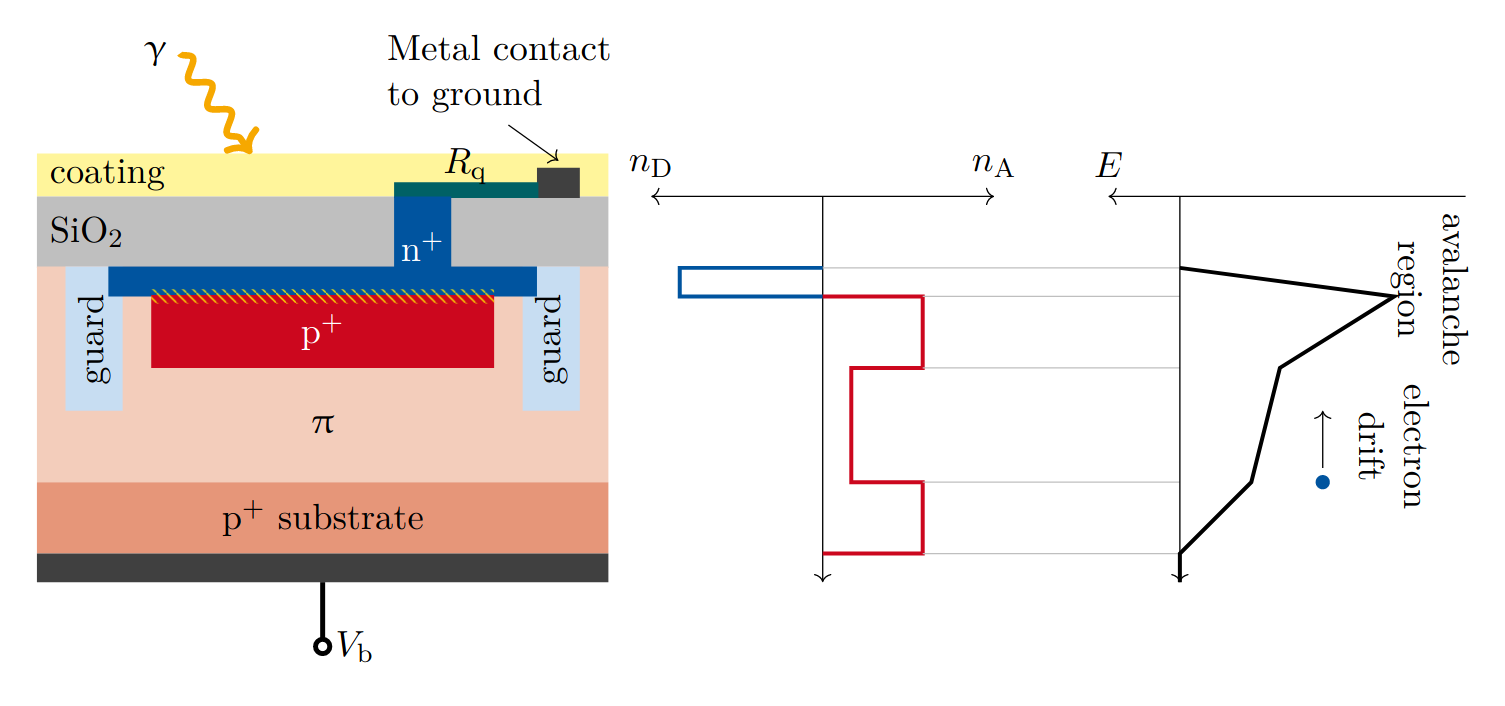
\includegraphics[width=1.\textwidth]{pictures/pin_diode}
	\caption[Illustration of a APD.]{Composition of an avalanche photodiode with the bias voltage $V_\text{B}$ applied in the reverse direction. Between the contact to the ground and the strongly doped $n^+$ layer is the quenching resistor $R_\text{q}$ connected in series. Next to the $n^+$ layer is a strongly doped $p^+$ layer. In the region of these two layers is the electric field, shown in the right figure, the strongest. There, an electron or hole can initiate an avalanche. After the $p^+$ layer is an intrinsic weakly doped $\pi$ layer. This layer increases the sensitive volume of the diode. If a electron-hole pair is created, it gets separated by the electric field. The hole drifts towards the multiplication region and can start an avalanche. The next layer is a $p^+$ layer, which connects to a metal connector and high voltage. The picture in the middle illustrates the number of donators $n_D$ ad acceptors $n_A$, and the last picture illustrates the field strength at the different regions of the \ac{apd}. \cite{}}
	\label{fig:pin_diode}
\end{figure}

%When a reverse bias voltage is applied to the \ac{apd}, the electric field between the $n^+$ and $p^+$ layers is strong enough that a created $eh$-pair creates more $eh$-pairs, resulting in an avalanche.
%For this avalanche process to be possible the reverse bias voltage must be at or above the breakdown voltage of the \ac{apd}.
%With such a bias voltage applied, the \ac{apd} operates in the Geiger mode and the avalanche is then self-sustaining.
%This results in a macroscopic signal and makes the detection of single photons possible.
%Therefore these diodes are also called \ac{spad}.
%To stop the avalanche, a quenching resistor is connected in series with the \ac{spad}.
%With an increasing current signal flowing through the quenching resistor, the voltage drop at this resistor increases, and thus the bias voltage at the \ac{spad} decreases.
%When the bias voltage drops under the breakdown voltage, the avalanche is no longer self-sustaining and stops.
%Thus the signal amplitude of a \ac{spad} is always similar, independent of how many photons arrive at the same moment.

In \acp{sipm}, hundreds to thousands of \acp{spad} are connected in parallel, each with a high-resistance quenching resistor in series. 
Usually, the \ac{spad} pixels are placed in a rectangular form with an edge length of a few \si{\milli\meter}.
\autoref{fig:sipm_closeup} shows a picture of a \ac{sipm} and one picture of a single pixel of a \ac{sipm}.
Due to the property of the \acp{spad} that the output signal is always similar for each \ac{spad}, the output signal of a \ac{sipm} is the output signal of one \ac{spad} multiplicated by the number of triggered \acp{spad}.
Therefore, if the number of photons arriving simultaneously at a \ac{sipm} is low enough that the probability of one \ac{spad} being hit by two or more photons is low, one can count photons with a \ac{sipm}.
This and the relatively low cost, high durability, and impassivity to magnetic fields make them a good option for photodetection for the \ac{sbt} and similar detectors.
However, due to the sensitivity down to single photons, also $eh$-pairs created by thermal excitation will cause signals indistinguishable from signals caused by photons.
These signals are called \ac{dc}.



%In the following different properties of \acp{sipm} are presented, beginning with the signal shape of a single \ac{spad} and of a \ac{sipm}.


%\paragraph{The signal shape} of a \acp{spad} starts with a fast exponential rise with the time constant 
%\begin{align}
%	\tau_\text{rise}&=R_\text{S}\cdot C_\text{d}
%\end{align}
%with the resistance $R_\text{rise}$ and capacitance $C_\text{d}$ of the \ac{spad} \cite{HAMA_mppc}.
%After the signal reached its maximum current at around 
%\begin{align}
%	I_\text{max}&\approx \frac{V_\text{ov}}{R_\text{q}}
%\end{align}
%the quenching and recharging of the \ac{spad} starts.
%Thus the current signal decreases again exponentially.
%The time constant for the signal decay
%\begin{align}
%	\tau_\text{decay} &= R_\text{q}\cdot C_\text{d}
%\end{align}
%depends on the capacitance $C_\text{d}$ of the \ac{spad} and the quenching resistor $R_\text{q}$ \cite{HAMA_mppc}.
%This signal develpment is shown in \autoref{fig:spad_signal_shape}.
%\begin{figure}
%	\centering
%	\includegraphics[width=0.75\textwidth]{pictures/spad_signal_shape}
%	\caption[SPAD signal shape]{Single photon avalanche diode signal shape. The exponential rise with the time constant $R_\text{S}\cdot C_\text{d}$ is followed by the exponential decay with the time constants $R_\text{q}\cdot C_\text{d}$. The maximum of the current signal is at approximately $V_\text{ov}/R_\text{q}$ \cite{HAMA_mppc}}
%	\label{fig:spad_signal_shape}
%\end{figure}

%When multiple \acp{spad} in a \ac{sipm} are triggered, the output signal will be the summation of the signals from all triggered \acp{spad}.
%Besides the number of triggered \acp{spad}, the time difference between the signals from the single \acp{spad} influences the signal.
%In the case, that all \acp{spad} are triggered at the same time, the \ac{sipm} signal will have the shape of a \ac{spad} signal scaled up by the factor of the number of triggered \acp{spad}.
%If the signals form the individual \acp{spad} have a small difference in time, the \ac{sipm} signal will become broader.



An essential property of a \ac{sipm} is the gain $G$.
It describes the number of charge carriers released in each avalanche.
Due to the quenching, this parameter is well-defined \cite{}.
It can be calculated from the applied voltage $U_\text{bias}$, the breakdown voltage $U_\text{bd}$ and the capacitance $C_\text{d}$ of a \ac{spad} with
\begin{align}
	G &= \frac{(V_\text{bias}- V_\text{bd})\cdot C_\text{d}}{\text{e}}.
\end{align}
Here, e represents the charge of one electron.
Usually, the gain is in the order of $10^5$ to $10^7$ \cite{nucl}.
Since the breakdown voltage of different \acp{sipm} of the same model can differ slightly, also the gain with the same bias voltage can differ.

The next section presents the \ac{asic} used to amplify the \ac{sipm} signals.
%\paragraph{The noise} in \acp{sipm} can be sorted into two categories.
%The first is primary noise, it describes the triggering of avalanches by thermaly created $eh$-pairs and not by incident photons.
%Because the rate of theses thermaly caused events increases and decreases with the temperature, by controling the temperatur one can influence and decrease the rate of primary noise events.
%The second category is the correlated noise.
%It includes all events triggered by a primary event.
%This correlated noise does have two causes.
%One cause is the trapping and releasing of charge carriers from the avalanche. 
%When the time between the trapping and releasing is long enough, the avalanche of the primary event stoped and the released carrier can trigger another avalanche.


\section{The eMUSIC board}
Since the signals of the \acp{sipm} are tiny, they need to be amplified.
For this purpose, the \ac{emusic} \ac{asic} by Scientifica was chosen, and a custom \ac{pcb} housing the \ac{emusic} \ac{asic}, from here on called \ac{emusic} board, was designed by the electrical engineers of the University of Freiburg.
In the following first, the \ac{asic} itself and afterward, the \ac{emusic} board will be presented.

\paragraph{The eMUSIC ASIC} was developed by Scientifica for the readout of \acp{sipm}.
It is mainly an amplifier and a shaper, but it also offers other options like digital trigger signals if the signal crosses an adjustable threshold.
The \ac{asic}\'s block diagram is shown in \autoref{fig:emusic_block_diagram}.
\begin{figure}
	\centering
	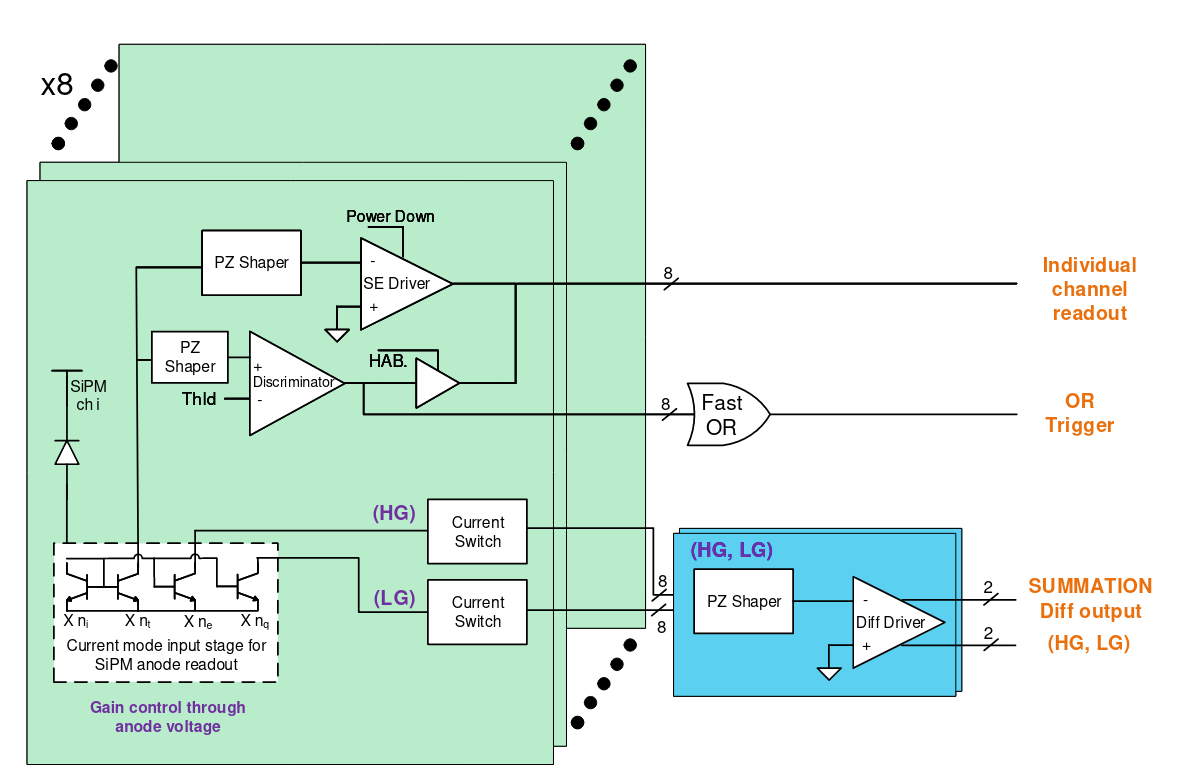
\includegraphics[width=1.\textwidth]{pictures/emusic_block_diagram.png}
	\caption[eMUSIC block diagram]{The block diagram of the \ac{emusic} \ac{asic}. At the input is the current mode input stage, which can also set an offset voltage on the input to adjust the overvoltage channel by channel. The signal then gets shaped by the pole-zero cancellation shaper and amplified and can be read out for each channel as a single-ended signal. The discriminator can set a threshold to create a digital signal which can be read out channel by channel instead of the analog output signal. A fast OR output can also be used to put out a digital OR of all eight discriminator outputs. With the summation outputs, one can put out the sum of an arbitrary set of channels with two gains as differential signals. \cite{gomez}}
	\label{fig:emusic_block_diagram}
\end{figure}
It has eight input channels, each equipped with a $\approx\SI{1}{\volt}$ anode voltage control to equalize the applied overvoltage between the different channels.
Because the \acp{sipm} deliver a charge signal, each channel has a current mode input stage.
The \ac{emusic} \ac{asic} was designed to have a low input transimpedance but provides the option of a high transimpedance mode with which the gain can be increased.
Each individual channel has a bandwidth of \SI{150}{\mega\hertz} and a pole-zero cancellation, schematics shown in \autoref{fig:emusic_pole_zero}, with two adjustable resistors and an adjustable capacitor.
It can be used to decrease the \ac{fwhm} of the output signal to below $\SI{10}{\nano\second}$.
But a smaller width also attenuates the amplitude of the signal.
The resistor has eight possible values it can be set to, and the capacitor has thirty-two different steps.
Although the \ac{emusic} provides the option of a lower attenuation mode of the pole-zero cancellation, a compromise between smaller signal width and higher amplitude should be chosen depending on one's needs.
Alternatively, the pole-zero cancellation can be disabled completely, resulting in the highest signal amplitude possible with the \ac{emusic} but also in the longest signal.
The signal after the shaper can be put out with an analog output for each channel.
\begin{figure}
	\centering
	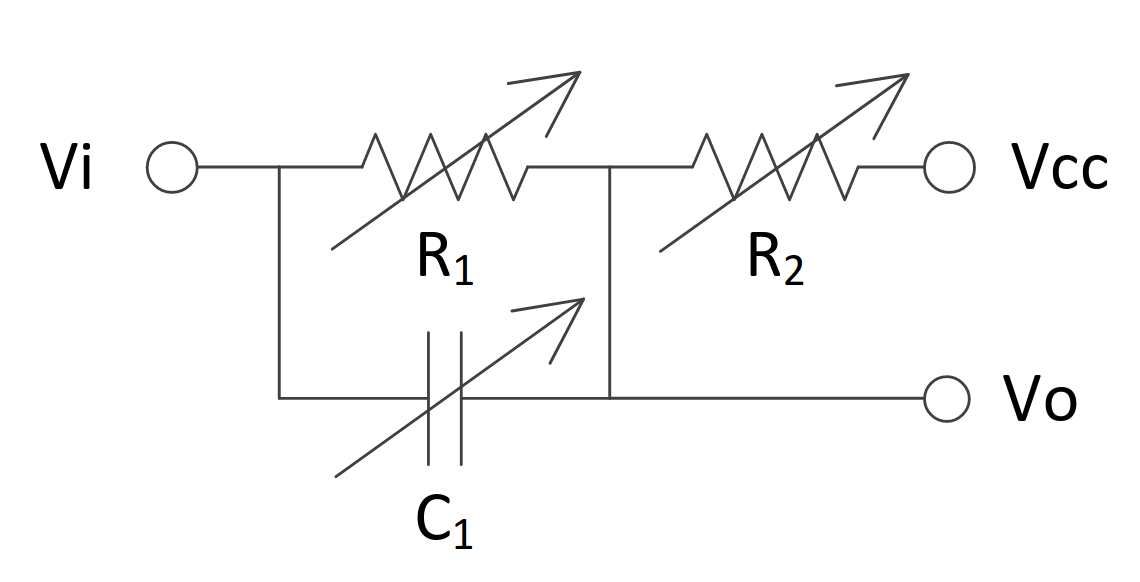
\includegraphics[width=0.5\textwidth]{pictures/emusic_pole_zero.png}
	\caption[eMUSIC pole-zero cancellation]{Sketch of a pole-zero cancellation with adjustable resistors and capacitor, the input voltage $\text{V}_\text{i}$, the output voltage $\text{V}_\text{o}$, and the operation voltage $\text{V}_\text{cc}$. \cite{gomez}}
	\label{fig:emusic_pole_zero}
\end{figure}

Each channel also possesses a discriminator with an adjustable threshold to create a channel-by-channel trigger signal.
These logical signals can be either put out by using the individual output of the channel for the digital signal instead of the analog waveform or by using the fast OR of all channels.
This fast OR allows, for example, the external triggering of the digitizer, which then digitizes the analog waveforms if the waveform of one or more channels surpasses the threshold.
The dynamic range of the output for the single-ended signals is \SI{1}{\volt} if the load on the output is \SI{50}{\ohm} and \SI{2}{\volt} if a high impedance load is used on the output.
Using the low transimpedance mode, the gain of the single-ended output is \SI{180}{\ohm}, and with the high transimpedance mode, it is \SI{480}{\ohm}.
Over the first half of the dynamic range, the response of the \ac{emusic} is linear, and over the second half, it is non-linear.

Besides the individual readout of the eight channels, the \ac{emusic} can sum up the signal of an arbitrary set of channels with both high and low gain and put them out via two differential outputs.
The bandwidth of this summation output is \SI{500}{\mega\hertz}, and the output range is \SI{1.25}{\volt}.
Depending on whether the high or low transimpedance is used, the gain of the high gain summation is \SI{690}{\ohm} or \SI{90}{\ohm} and \SI{315}{\ohm} or \SI{45}{\ohm} for the low gain summation. 
The response of the summation output is linear over the dynamic range.

Besides choosing the channels for summation, also each of the eight single-ended outputs can be individually turned on and off.
Another important option that can be configured is the adjustment of the output DC offset to maximize the rail-to-rail voltage swing.

\paragraphe{The trigger threshold} for the digital outputs can be set with two parameters.
The first one is the bandgap voltage $V_\text{bg}$ of the comparators, which can be adjusted in eight steps between \SI{487.22}{\milli\volt} and \SI{2436.8}{\milli\volt}.
The second parameter sets the \ac{dac} value $N_\text{DAC}$ for the comparators.
It can be set to \ac{dac} counts from 0 to 511.
The finer threshold steps $V_\text{fine}$ can be calculated with
\begin{align}
	V_\text{fine}&=\SI{1637.79}{\milli\volt} - N_\text{DAC}\cdot\SI{3.1445}{\milli\volt}.
\end{align}
With $V_\text{bg}$ and  of $V_\text{fine}$ or $N_\text{DAC}$, the final threshold
\begin{align}
	V_\text{th}&= 1.5\cdot V_\text{bg} - 0.5\cdot V_\text{fine}\\
		   &= 1.5\cdot V_\text{bg} - 0.5\cdot (\SI{1637.79}{\milli\volt} - N_\text{DAC}\cdot\SI{3.1445}{\milli\volt})
\end{align}
can be calculated.

\paragraph{The eMUSIC board} was designed at the University of Freiburg.
A graphic of the board is shown in \autoref{fig:emusic_board}.
Its heart is the \ac{emusic} \ac{asic} (U1).
In order to program the \ac{asic}, the ATmega328P-AU microchip (U4) is placed on the board.
The microchip can be programmed with the XXXX software by XXXXX and the XXXXX, which is connected to the computer via USB and can be plugged into the J4 connector on the \ac{emusic} board.
After programming the microchip, it only has to be programmed again if the reset button SW1 is pressed.
Then the \ac{emusic} \ac{asic} can be configured by using a TTL-to-USB adapter connected to a computer and the P3 connector, and the software of the minimusic board.
The minimusic board is a commercial product using the \ac{emusic} \ac{asic}.
Due to the \ac{emusic} board being designed to work with the minimusic software, one avoids the need to write software and also has the security that the used software was tested and is working correctly.
Two functions of the minimusic software are not usable on the \ac{emusic} board, the calibration of the threshold and the calibration of the DC offset on the outputs.
Therefore these two need to be set by the user.

The high voltage for the \acp{sipm} can be supplied via the P2 SMA connector.
On the backside of the \ac{pcb} is an LSHM-150-XX.-XXX-DV-AN-XX connector located to connect the board to the \ac{sipm} board.
Via this connector, the high voltage is brought to the \acp{sipm}, and the signals are brought to the \ac{emusic} inputs.
The eight single-ended outputs can be read out by the SMA connectors K1 to K8.
The fast OR signal can be read out via the K9 connector.
Both the high and low gain differential summation outputs are connected to the pins of the J6 connector.

The board also provides the possibility via the P1 connector to power the six LEDs soldered onto the \ac{sipm} boards.
However, the usage of this is not advised since this will introduce interferences into the signals.

The amplified single-ended output signals then can be digitized.
For this task, the GANDALF module was chosen, which is described in the next section.

\begin{figure}
	\centering
	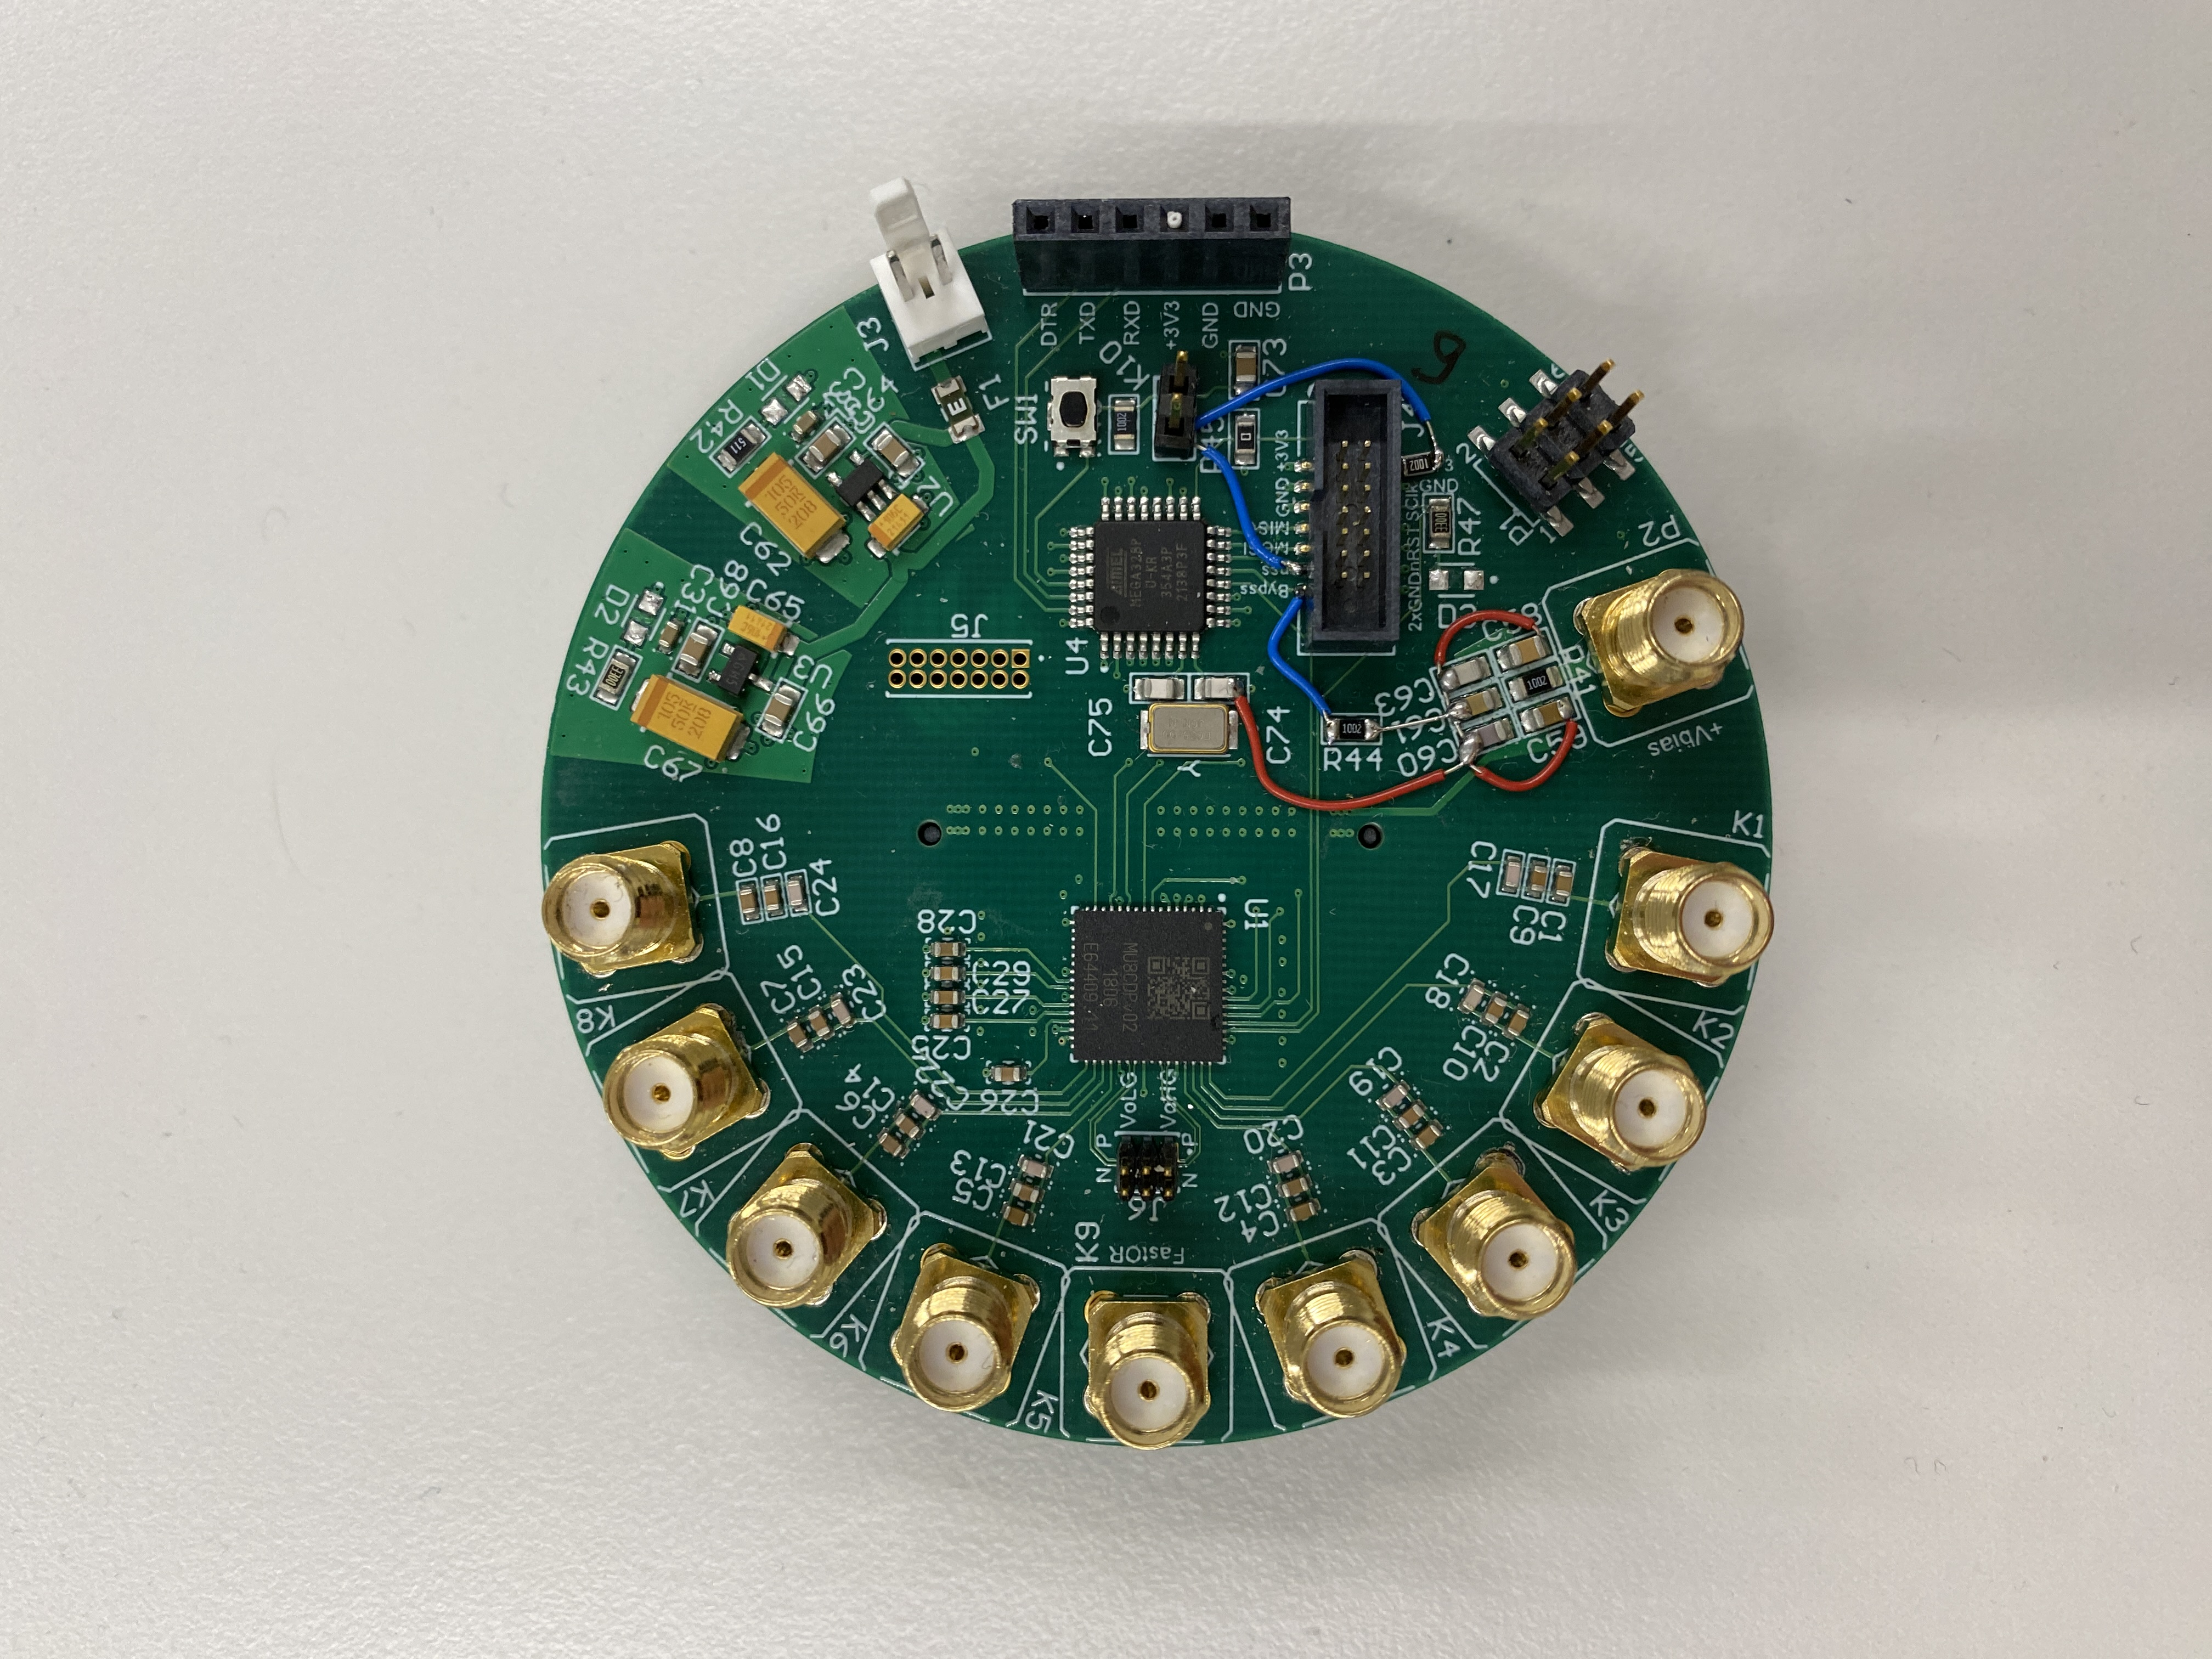
\includegraphics[width=1.\textwidth]{pictures/emusic_board}
	\caption[eMUSIC Board]{Picture of the \ac{emusic} board with the \ac{emusic} \ac{asic}, the eight single-ended channel-by-channel SMA signal outputs, the SMA fast OR output, the differential signal output, the SMA connector for the high voltage supply of the \acp{sipm}, and the connectors to program and power the board.}
	\label{fig:emusic_board}
\end{figure}





\section{The GANDALF Module}
The amplified and shaped output signal of the \ac{emusic} \ac{asic} needs to be digitized.
This step is done by GANDALF modules.
Originally developed at the University of Freiburg for the \ac{compass} experiment, it has a modular design to fill different roles in the experiments \ac{daq}.
Using mezzanine cards, different signal, clock, and trigger inputs can be chosen.
In the following, the GANDALF module will be introduced.
The mezzanine cards not used in this work are therefore only mentioned but not presented in detail.
An overview of a GANDALF module is shown in \autoref{fig:gandalf_overview}.
\begin{figure}
	\centering
	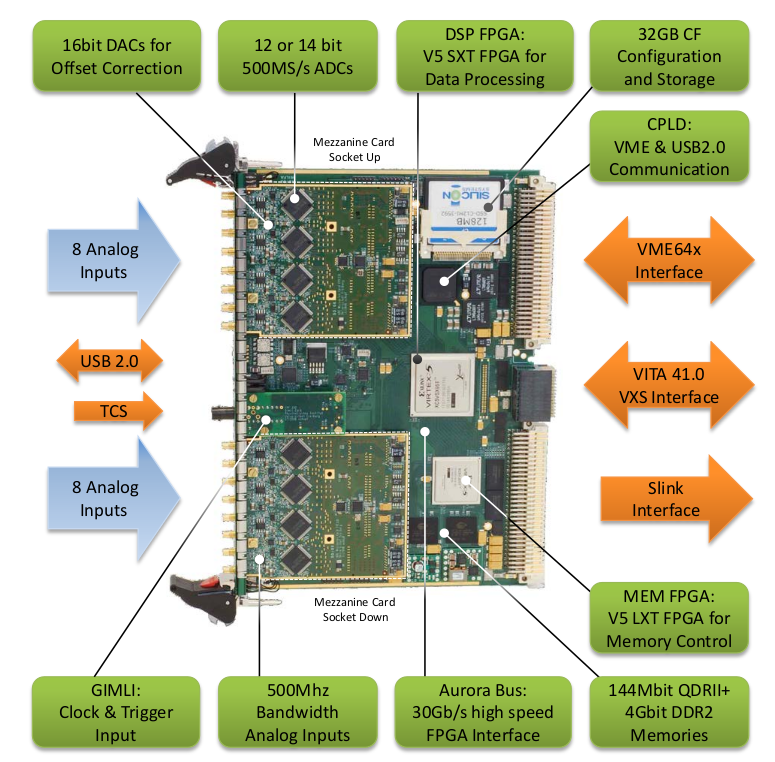
\includegraphics[width=.8\textwidth]{pictures/gandalf_overview.png}
	\caption[Overview of the GANDALF module]{Overview of the GANDALF module equipped with Analog Mezzanine Cards (AMCs) and the fiber Gimli mezzanine card for clock and trigger input. The analog waveforms are digitized by the AMCs, and the digitized data is processed by the DSP FPGA. The MEM FPGA handles the memory of the processed data, which can be transferred to a computer via the USB interface on the front of the VME or S-Link interfaces on the backplane. \cite{herrmann}}
	\label{fig:gandalf_overview}
\end{figure}

\subsection{Input Mezzanine Cards}
The GANDALF module has two mezzanine card slots for input signals.
For these slots, three different mezzanine cards were developed, \ac{amc}, \ac{dmc}, and \ac{omc}.
First, the last two mezzanine cards are shortly presented for completeness but are not relevant to the work done in this thesis.

\paragraph{The \ac{dmc}} has 64 digital inputs. 
%A picture of it is shown in \autoref{fig:dmc}.
Using either the LVDS or the LVPECL signal standard, one can use the DSP-\ac{fpga} logic for tasks like trigger decisions, time-to-digital conversion, or pattern generators, to name a few.
By changing the direction of the input buffer on the \ac{dmc} \ac{pcb}, the 64 channels of the \ac{dmc} can be used as outputs instead of inputs.

\paragraph{The \ac{omc}} has four \SI{3.25}{\giga\bit\per\second} transceivers to receive digital information, which can be further processed by the DSP-\ac{fpga}.
With this mezzanine card, the GANDALF can be used, for example, to merge data or as a concentrator.
%A picture of a \ac{omc} is shown in \autoref{fig:omc}.

\paragraph{The \ac{amc}} is designed to digitize analog input signals.
For digitization, eight \ac{adc} are used.
There are \ac{amc} with two different \ac{adc} available.
One is the \textit{ADS5463}, with \SI{12}{\bit} and up to \SI{500}{\mega\sample\per\second}, and the other is the \textit{ADS5474} which samples with up to \SI{400}{\mega\sample\per\second} at \SI{14}{\bit}.
The \ac{enob} of both \acp{adc} are \SI{10.4}{\bit} and \SI{11.2}{\bit}, respectively.
Each \ac{amc} has eight SMC connectors for the inputs.
There are \ac{amc} operating in \textit{normal mode}, meaning each SMC connector is connected to one \ac{adc}, resulting in eight channels with up to \SI{500}{\mega\sample\per\second} or \SI{400}{\mega\sample\per\second} per \ac{amc}.
In order to increase the sampling frequency, \acp{amc} which operate in the \textit{interleaved mode} were built.
On these \acp{amc}, four inputs are connected to two \ac{adc}s each, and therefore every second SMC connector is a dead end.
The clock signals which provide the sample tact for the two \acp{adc} of one channel have \SI{180}{\degree} phase offset with respect to each other.
By this, the sampling frequency is doubled to up to \SI{1}{\giga\sample\per\second} or \SI{800}{\mega\sample\per\second}, but the number of channels per \ac{amc} is reduced from eight to four.
The dynamic input range of the \ac{amc} is \SI{4.4}{\vpp} and can be shifted from the negative unipolar range \SIrange{-4.4}{0}{\volt} up to the bipolar range \SIrange{-2.2}{2.2}{\volt}.
This shifting is done by an \textit{AD5665R}, a \SI{16}{\bit} \ac{dac}.
The dynamic range was chosen because in the COMPASS experiment, for which the GANDALF was developed, negative voltage pulses created by \acp{pmt} needed to be digitized.
However, because the used \acp{adc} expect positive differential signals, inverting operational amplifiers are used to change the polarity of the signal.
By changing the gain of the amplifiers, one can decrease the input range and therefore increase the amplitude resolution.
The \acp{amc} used in this thesis are \SI{12}{\bit} \acp{amc} in the \textit{interleaved mode} and a dynamic range of \SI{2.2}{\vpp}.


\subsection{GIMLI Mezzanine Cards}
The third mezzanine card slot is for the GIMLI mezzanine cards, which are responsible for the clock and external trigger signals.
For this mezzanine card, three different options were developed.
One GIMLI card, which takes the clock and trigger from the backplane, if one wants to use the create to distribute the signals.
The fiber GIMLI has one fiber input to receive the clock and trigger via optical fiber.
And the copper GIMLI, which was used for this work and is presented in the following.

The copper GIMLI, shown in \autoref{fig:copper_gimli}, provides the option to use an external or an internal clock.
If only one GANDALF module is used, the internal \SI{20}{\mega\hertz} clock of the copper GIMLI can be used.
It is provided by an onboard oven-controlled oscillator (OCXO) with a jitter of less than \SI{2.3}{\pico\second}.
In case two or more GANDALFs are used, an external clock is required to ensure a synchronized clock on all GANDALF modules.
For this case, the copper GIMLI has a LEMO connector as input for an external clock with \ac{nim} signal standard.
Via a second LEMO connector, an external \ac{nim} trigger signal can be connected to the GANDALF module.

\begin{figure}
	\centering
	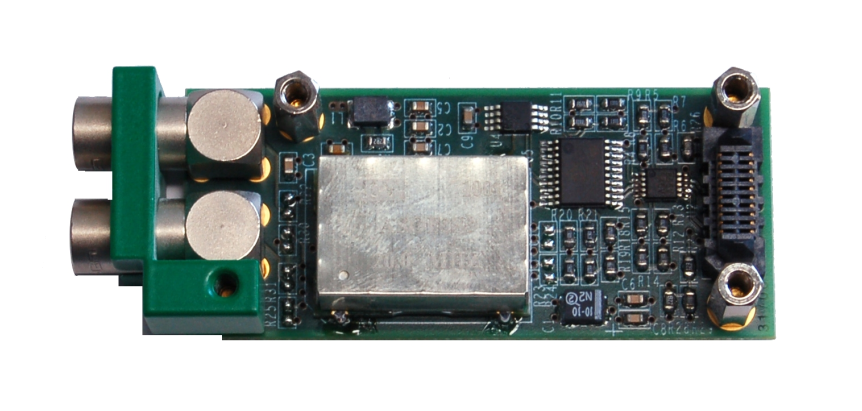
\includegraphics[width=.5\textwidth]{pictures/copper_gimli.png}
	\caption[Copper GIMLI]{Picture of the copper GIMLI with an internal \SI{20}{\mega\hertz} clock generated by an onboard oven-controlled oscillator. With the LEMO connectors external clock and trigger \ac{nim} signals can be provided for the GANDALF. \cite{herrmann}}
	\label{fig:copper_gimli}
\end{figure}



\subsection{Usage of the GANDALF with \acp{sipm}}
In this work, the GANDALF was used for digitizing the output signal of the \ac{emusic} \ac{asic}.
As mentioned above in \autoref{sec:emusic}, these signals have a positive polarity.
But because the GANDALF was designed for the digitization and processing of negative voltage pulses created by a \ac{pmt}, this caused some problems.
Since after the inverting operational amplifiers in the GANDALF, the \ac{sipm} signals have a negative polarity, the input voltage range needs to be chosen to be bipolar and around \SIrange{-1.1}{1.1}{\volt}.
%In order to get this input range the baseline at \SI{0}{\volt} would need to be set to \SI{2047}{\adcu}.
%For unknown reasons the programm which configeres the \acp{dac} to set the baseline to a \si{\adcu} value selectable by the user will set the baseline to a maximum of around \SI{1400}{\adcu}.
%With $\frac{2.2}{2^12}\,\si{\volt\per\adcu} = \SI{0.537}{\milli\volt\per\adcu}$ the range of the inverted signal is \SI{1400}{\adcu} which corresponds to approximately \SI{752}{\milli\volt}.
%Should this range be not enough, one needs to either try to find the source of the problem and fix it or decrease the amplification of the \ac{emusic} \ac{asic}.
%The next problem regards the self-trigger of the GANDALF.
Also, the self-trigger of the GANDALF needed to be adjusted.
It functions via samples over threshold.
The user can set a threshold and a number of consecutive samples which need to be over the threshold for the GANDALF to trigger an event.
Since after the inverting of the positive signals, the signals have a negative polarity, and the threshold needs to be set to a lower ADC value than the baseline.
In addition to that, the sample over threshold condition in the GANDALF firmware needed to be inverted to trigger if a number of consecutive samples were below the threshold.
The new firmware with the inverted trigger condition was tested and worked as intended, with the exception of one bug.
If the data rate from the GANDALF to the \ac{daq} computer exceeds the maximum possible data rate, \SI{20}{\mega\byte\per\second} in the case of the USB interface, incomplete events will be written down to disk.
This is most likely caused by a missing VHDL file that was not included in the new firmware and which would, in case the buffer of the GANDALF is completely filled, prevent the GANDALF from sending incomplete events to the computer.
For the intended use of this bug should not be a problem since the data rate is expected to be way below the possible \SI{20}{\mega\byte\per\second}.
